%%%%%%%%%%%%%%%%%%%%%%%%%%%%%%%%%%%%%%%%%
% Quiz #1 Template
% LaTeX Template
% By: Ryan Grove
%%%%%%%%%%%%%%%%%%%%%%%%%%%%%%%%%%%%%%%%%

%----------------------------------------------------------------------------------------
%	PACKAGES AND OTHER DOCUMENT CONFIGURATIONS
%----------------------------------------------------------------------------------------

\documentclass[paper=a4, fontsize=11pt]{scrartcl} % A4 paper and 11pt font size

\usepackage[T1]{fontenc} % Use 8-bit encoding that has 256 glyphs
\usepackage{fourier} % Use the Adobe Utopia font for the document - comment this line to return to the LaTeX default
\usepackage[english]{babel} % English language/hyphenation
\usepackage{amsmath,amsfonts,amsthm} % Math packages

\usepackage{lipsum} % Used for inserting dummy 'Lorem ipsum' text into the template

\usepackage{sectsty} % Allows customizing section commands
\allsectionsfont{\centering \normalfont\scshape} % Make all sections centered, the default font and small caps

\usepackage{fancyhdr} % Custom headers and footers
\pagestyle{fancyplain} % Makes all pages in the document conform to the custom headers and footers
\fancyhead{} % No page header - if you want one, create it in the same way as the footers below
\fancyfoot[L]{} % Empty left footer
\fancyfoot[C]{} % Empty center footer
%\fancyfoot[R]{\thepage} % Page numbering for right footer
\renewcommand{\headrulewidth}{0pt} % Remove header underlines
\renewcommand{\footrulewidth}{0pt} % Remove footer underlines
\setlength{\headheight}{13.6pt} % Customize the height of the header

\numberwithin{equation}{section} % Number equations within sections (i.e. 1.1, 1.2, 2.1, 2.2 instead of 1, 2, 3, 4)
\numberwithin{figure}{section} % Number figures within sections (i.e. 1.1, 1.2, 2.1, 2.2 instead of 1, 2, 3, 4)
\numberwithin{table}{section} % Number tables within sections (i.e. 1.1, 1.2, 2.1, 2.2 instead of 1, 2, 3, 4)

\setlength\parindent{0pt} % Removes all indentation from paragraphs - comment this line for an assignment with lots of text

\usepackage{lastpage}
\usepackage{fancyhdr}
\cfoot{\thepage\ of \pageref{LastPage}}

\def\v{\hbox{$\mathbf v$}}
\def\w{\hbox{$\mathbf w$}}
\def\u{\hbox{$\mathbf u$}}
\def\x{\hbox{$\textbf{x}$}}
\def\z{\hbox{$\mathbf z$}}
\def\a{\hbox{$\mathbf a$}}
\def\b{\hbox{$\mathbf b$}}
\def\L{\hbox{$\mathcal L$}}
\def\C{\hbox{$\mathbb C$}}
\def\B{\hbox{$\mathcal B$}}
\def\R{\hbox{$\mathbb R$}}
\def\X{\hbox{$\underline X$}}
\def\Q{\hbox{$\mathbb Q$}}
\def\R{\hbox{$\mathbb R$}}
\def\N{\hbox{$\mathbb N$}}
\def\C{\hbox{$\mathbb C$}}
\def\0{\hbox{$\mathbf 0$}}
\def\Y{\hbox{$\underline Y$}}
\def\a{\hbox{$\mathbf a$}}
\def\u{\hbox{$\mathbf u$}}
\def\w{\hbox{$\mathbf w$}}
\def\y{\hbox{$\mathbf y$}}
\def\X{\hbox{$\underline X$}}
\def\dd{\hbox{$\partial $}}
\def\B{\hbox{$\mathcal B$}}
\def\F{\hbox{$\mathcal F$}}
\def\L{\hbox{$\mathcal L$}}
\def\M{\hbox{$\mathcal M$}}
\def\D{\hbox{$\mathscr {D}$}}
\def\RR{\hbox{$\mathscr{R}$}}
\def\I{\hbox{$\mathcal I$}}

\usepackage{amssymb}
%\theoremstyle{plain}
\usepackage[margin = .75in]{geometry}
\newtheorem{claim}{Claim}
\newtheorem{theorem}{Theorem}[section]
\newtheorem{lemma}[theorem]{Lemma}
\newtheorem{proposition}[theorem]{Proposition}
\newtheorem{corollary}[theorem]{Corollary}
\newtheorem{problem}[theorem]{Problem}
%\theoremstyle{definition}
\newtheorem{definition}[theorem]{Definition}
%\theoremstyle{remark}
\newtheorem{remark}[theorem]{Remark}
\newtheorem{remarks}[theorem]{Remarks}
\newtheorem{example}[theorem]{Example}
\newcommand{\ds}{\displaystyle}
\newcommand{\ZZ}{\mathbb{Z}}
\newcommand{\QQ}{\mathbb{Q}}
\newcommand{\e}{\varepsilon}
\newcommand{\bbf}{\textbf}
\newcommand{\p}{\parallel}
\usepackage{color}
\newcommand{\field}[1]{\mathbb{#1}}
\usepackage{amsmath}
\usepackage{amsthm}
\usepackage{amssymb}
\usepackage{mathrsfs}
\usepackage{cancel}
\usepackage{upgreek}
\usepackage{graphicx}
\usepackage{multirow}
\usepackage{setspace}
\usepackage{url}
\usepackage{subfigure}
\usepackage{enumerate}
\usepackage{cases}
\usepackage{mathrsfs}
\usepackage{rotating}

%----------------------------------------------------------------------------------------
%	TITLE SECTION
%----------------------------------------------------------------------------------------

\newcommand{\horrule}[1]{\rule{\linewidth}{#1}} % Create horizontal rule command with 1 argument of height

\title{	
\normalfont \normalsize 
\textsc{Ryan Grove, Clemson University, MATH1080 - 9} \\ [25pt] % Your name, university, class
\horrule{0.5pt} \\[0.4cm] % Thin top horizontal rule
\huge Section 6.3: Volumes by Cylindrical Shells \\ % The assignment title
\horrule{2pt} \\[0.5cm] % Thick bottom horizontal rule
}

\author{Date:} % The due date

\date{\normalsize January 13, 2016} % A custom date

\begin{document}

\maketitle % Print the title

\begin{flushleft}
\begin{tabular}{l l}
Name: \rule{3.2in}{.01cm}  & {}%Table number: \rule{1in}{.01cm}\\
\end{tabular}
\end{flushleft}

%----------------------------------------------------------------------------------------
%	Lecture
%----------------------------------------------------------------------------------------

\section*{\textbf{Lecture:}}

Some volume problems are very difficult to handle by the methods of the preceding section (Disk/Washer). Consider the problem of finding the volume of the solid obtained by rotating about the $y-$axis the region bounded by $y=2x^2-x^3$ and $y=0$. 
\[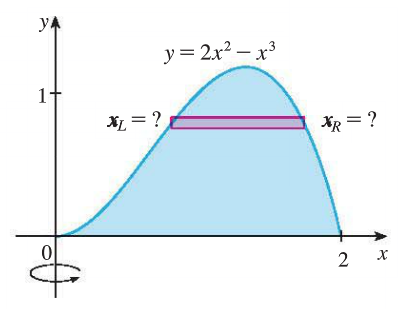
\includegraphics[scale=0.4]{6-3pic1.png}\]
If we slice perpendicular to the $y-$axis (i.e. horizontal slice), we get a washer. But to compute the inner radius and the outer radius of the washer, we'd have to solve the cubic equation $y=2x^2 - x^3$ for $x$ in terms of $y$; that's not easy.\\
\indent

Fortunately, there is an alternate method, called the \underline{\hspace{1in}} \underline{\hspace{1in}} (or method of cylindrical shells), that is easier to use in such a case. Figure 2 shows a cylindrical shell with inner radius $r_1$, outer radius $r_2$, and height $h$. Its volume $V$ is calculated by subtracting the volume $V_1$ of the inner cylinder from the volume $V_2$ of the outer cylinder:\\
\indent

\quad \quad \quad 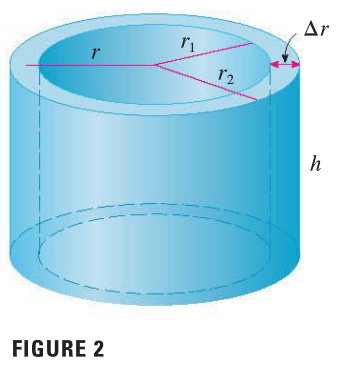
\includegraphics[scale=0.4]{6-3pic2.png}\\
\indent

If we let $\Delta r= r_2-r_1$ (the thickness of the shell) and $r=\frac{1}{2}(r_2+r_1)$ (the average radius of the shell), then this formula of a cylindrical shell becomes

\[\underline{\hspace{1.5in}}\]
and it can be remembered as

\[\underline{\hspace{3in}}\]

\indent

Let $S$ be the solid obtained by rotating about the $y-$axis the region bounded by $y=f(x)$ [where $f(x)\geq 0$], $y=0$, $x=a$, and $x=b$, where $b>a\geq 0$.

\[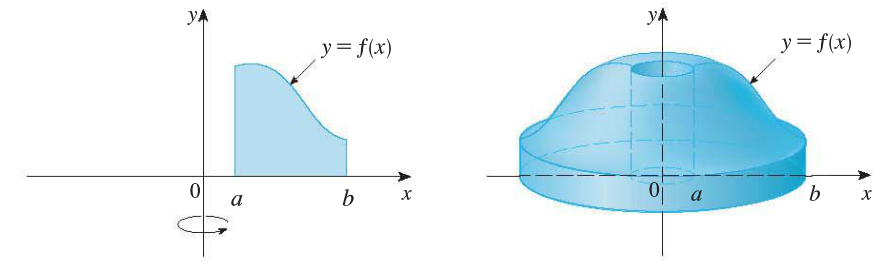
\includegraphics[scale=0.45]{6-3pic3.png}\]


\fbox{
  \parbox{\textwidth}{
  \vspace{5pt}
  
   The volume of the above solid obtained by rotating about the $y-$axis the region under the curve $y=f(x)$ from $a$ to $b$, is
   
   \[V = \underline{\hspace{1.5in}} \quad \quad \text{ where } 0\leq a \leq b\]
   
   }}
   \indent\\
   \indent
   
   %\fbox{
%  \parbox{\textwidth}{
%  \vspace{5pt}

\underline{Volume via Shell Method}:

The volume of a solid via Shell Method, in general, is:

\[\ds\int_a^b \text{ } 2\pi  (\text{radius}) \text{ } \cdot \text{ }(\text{height}) \text{ } dx \quad \text{OR} \quad \ds\int_c^d \text{ }2\pi (\text{radius}) \text{ } \cdot \text{ } (\text{height})\text{ } dy.\]
\indent\\
\indent\\
\indent

where \textit{radius} = distance from axis of rotation to slice and \textit{height} = length of slice.\\
\indent

For Shell Method, a "slice" must be \underline{\hspace{1.15in}} to the axis of rotation.\\
\indent


   
\newpage

\underline{Example 1}: Find the volume of the solid obtained by rotating about the $y-axis$ the region bounded by $y=2x^2 - x^3$ and $y=0$.


\vspace{4.25in}

\section*{Disk/Washer Method vs. Shell Method}

\underline{Example 2}: Find the volume of the solid obtained by rotating about the $y-$axis the region between $y=x$ and $y=x^2$.


\newpage

\underline{Example 3}: Find the volume of the solid obtained by rotating about the $x-$axis the region under the curve $y=\sqrt{x}$ from $0$ to $1$.\\
\indent

\vspace{4.25in}


\underline{Example 4}: Find the volume of the solid obtained by rotating the region bounded by $y=x-x^2$ and $y=0$ about the line $x=2$.\\
\indent\\

%----------------------------------------------------------------------------------------

\end{document}